\input{preamble.tex}

\begin{document}
\pagestyle{fancy}
\fancyhead[L]{Seconde}
\fancyhead[C]{\textbf{DS n°7a - Vecteurs}}
\fancyhead[R]{\today}

\reversemarginpar

\null\vspace{-30pt}
Nom / Prénom : \\

Consignes particulières : 
\begin{itemize}[label=$\bullet$]
	\item 
	La calculatrice est \textbf{interdite}.
		\item 
	L'exercice \ref{exe:cours_a} peut être fait entièrement sur la feuille d'évaluation. 
	Écrire son nom avant de rendre le sujet pour qu'il soit corrigé.
	\item 
	Toute trace de recherche est prise en compte.
	%\item 
	%L'abbréviation $\tq$ signifie ``tel que''.
\end{itemize}

\hrule
\null\vspace{10pt}
Sauf mention contraire, on se place toujours dans un repère $(O, \vec{i}, \vec{j})$.

\exe{3}{
On donne $\vec{u}\pvec{6}{3}, \vec{v}\pvec{-2}{1}$ et $\vec{w}\pvec{8}{2}$. Compléter les phrases ci-dessous.
\begin{enumerate}[label=(\roman*),itemsep=5pt]
\item $\dfrac13 \vec{u} \pvec{\dots \dots}{\dots \dots}$ ;
\item $(\vec{u} - \vec{v}) \pvec{\dots \dots}{\dots \dots}$ ;
\item Les vecteurs $\vec{u}$ et $\vec{w}$ sont $\dots \dots$.
\end{enumerate}
}{exe:cours_a}{
\begin{enumerate}[label=(\roman*),itemsep=5pt]
\item $\dfrac13 \vec{u} \pvec{2}{1}$ ;
\item $(\vec{u} - \vec{v}) \pvec{8}{2}$ ;
\item Les vecteurs $\vec{u}$ et $\vec{w}$ sont non colinéaires (ou encore inégaux, de directions différentes, etc.).
\end{enumerate}
}

\exe{2}{
On considère les points $A(2;5), B(5;3), C(4;-1)$ et $D(7;-3)$.
Calculer les coordonnées des vecteurs $\vec{AB}$ et $\vec{CD}$. En déduire la nature du quadrilatère $ABCD$.
}{exe:pme1_a}{
$\vec{AB} \pvec{3}{-2}, \vec{CD} \pvec{3}{-2}, \vec{AB} = \vec{CD}$ donc $ABCD$ est un parallélogramme.
}

\exe{2}{
Donner les coordonnées des vecteurs ci-dessous :

\begin{center}

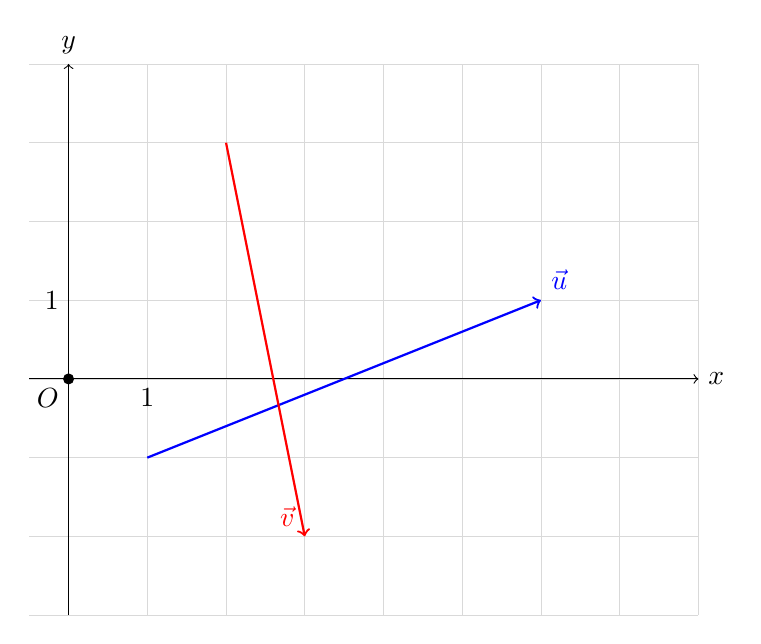
\begin{tikzpicture}[scale=1]

% Grille
\draw[step=1cm,gray!30,very thin] (-0.5,-3) grid (8,4);

% Axes
\draw[->] (-0.5,0) -- (8,0) node[right] {$x$};
\draw[->] (0,-3) -- (0,4) node[above] {$y$};

% Origine
\fill (0,0) circle (2pt) node[below left] {$O$};

% Graduation
\draw (1,0) node[below]{1};
\draw (0,1) node[left]{1};

% Vecteur u
\draw[->, thick, blue] (1,-1) -- (6,1) node[above right] {$\vec{u}$};

% Vecteur v
\draw[->, thick, red] (2,3) -- (3,-2) node[above left] {$\vec{v}$};

\end{tikzpicture}
\end{center}

}{exe:coord_a}{
$\vec{u}\pvec{5}{2}$ et $\vec{v}\pvec{1}{-5}$.
}

% récup manuel Magnard 2019
\exe{4}{
Soient $A, B$ et $C$ trois points non alignés. On construit les points $M, N$ et $P$ tels que :
\[ \vec{AM} = \dfrac13 \vec{AB} \qquad \vec{CN} = \dfrac13 \vec{CA} \et \vec{CP} = \dfrac13 \vec{BC} \]
\begin{enumerate}
\item Réaliser une figure ;
\item Exprimer $\vec{MN}$ en fonction de $\vec{BA}$ et $\vec{AC}$.
\item Exprimer $\vec{MP}$ en fonction de $\vec{BA}$ et $\vec{AC}$.
\item En déduire que les points $M, N$ et $P$ sont alignés.
\end{enumerate}
}{exe:chasles_a}{
\begin{enumerate}
\item 

\begin{center}
\begin{tikzpicture}

% --- Points ---
\coordinate (A) at (0,0);
\coordinate (B) at (3,3);
\coordinate (C) at (6,0);
\coordinate (M) at (1,1);
\coordinate (N) at (4,0);
\coordinate (P) at (7,-1);

% --- Segment ---
\draw[black, thick] (M) -- (P);

% --- Marques en croix ---
\foreach \P in {A,B,C,M,N,P}
{
    \draw[black] 
        ($(\P)+(-0.15,-0.15)$) -- ($(\P)+(0.15,0.15)$)
        ($(\P)+(-0.15,0.15)$) -- ($(\P)+(0.15,-0.15)$);
}

% --- Labels ---
\node[above] at (A) {A};
\node[above] at (B) {B};
\node[right] at (C) {C};
\node[left] at (M) {M};
\node[below] at (N) {N};
\node[right] at (P) {P};

\end{tikzpicture}
\end{center}

\item En utilisant la relation de Chasles et les données de l'énoncé :
\begin{align*}
\vec{MN} & = \vec{MA} + \vec{AC} + \vec{CN} \\
& = \dfrac13 \vec{BA} + \vec{AC} - \dfrac13 \vec{AC} \\
& = \dfrac13 \vec{BA} + \dfrac23 \vec{AC} .
\end{align*}
\item La démarche est identique :
\begin{align*}
\vec{MP} = \vec{MA} + \vec{AC} + \vec{CP} \\
& = \dfrac13 \vec{BA} + \vec{AC} + \dfrac13 \vec{BC} \\
& = \dfrac13 \vec{BA} + \vec{AC} + \dfrac13 (\vec{BA} + \vec{AB}) \\
& = \dfrac23 \vec{BA} + \dfrac43 \vec{AC}
\end{align*}
\item On a $\vec{MP} = 2 \vec{MN}$, les vecteurs $\vec{MP}$ et $\vec{MN}$ sont colinéaires, 
donc les points $M$, $N$ et $P$ sont alignés
\end{enumerate}
}

\exe{2}{
Dans chaque cas ci-dessous, déterminer si les droites $(AB)$ et $(CD)$ sont parallèles :
\begin{enumerate}[label=(\roman*)]
\item $A(5;-4), B(3; 1), C(-7 ; 2)$ et $D(-5 ; -2)$ ;
\item $A(-5; 1), B(9;-3), C(2 ; 2)$ et $D(9 ; 0)$   
\end{enumerate}
}{exe:det1_a}{
\begin{enumerate}[label=(\roman*)]
\item $\vec{AB}\pvec{-2}{5}$ et $\vec{CD}\pvec{2}{-4}$ donc $\det{\vec{AB}, \vec{CD}}=-2$, les droites $(AB)$ et $(CD)$ ne sont pas
parallèles.
\item $\vec{AB}\pvec{14}{-4}$ et $\vec{CD}\pvec{7}{-2}$ donc $\det{\vec{AB}, \vec{CD}}=0$, les droites $(AB)$ et $(CD)$ sont parallèles.
\end{enumerate}
}

\exe{2}{
Dans chaque cas ci-dessous, déterminer si les points $A, B$ et $C$ sont alignés.
\begin{enumerate}[label=(\roman*)]
\item $A(-4;-1), B(2; 2)$ et $C(6 ; 4)$ ;
\item $A(-2;5), B(1 ; -1)$ et $C(2, -7)$. 
\end{enumerate}
}{exe:det2_a}{
\begin{enumerate}[label=(\roman*)]
\item $\vec{AB}\pvec{6}{3}$ et $\vec{BC}\pvec{4}{2}$ donc $\det{\vec{AB}, \vec{BC}}=0$, les points $A, B$ et $C$ sont alignés.
\item $\vec{AB}\pvec{3}{-6}$ et $\vec{BC}\pvec{1}{-6}$ donc $\det{\vec{AB}, \vec{BC}}=-12$, les points $A, B$ et $C$ ne sont pas alignés.
\end{enumerate}
}

\exe{3}{
On donne $\vec{u}\pvec{3}{4}$.
\begin{enumerate}
\item Calculer la norme du vecteur $\vec{u}$.
\item Calculer la norme du vecteur $\dfrac15 \vec{u}$.
\item Soit $\vec{v} \pvec{1}{1}$. 
En vous inspirant de la question précédente, proposer un nombre $k \in \R$ tel que $\norm{k \vec{v}} = 1$.
\end{enumerate}
\textit{Ce procédé est appelé \og normalisation d'un vecteur \fg}.
}{exe:norm1_a}{
\begin{enumerate}
\item On trouve $\norm{\vec{u}} = \sqrt{3^2+4^2} = \sqrt{25} = 5$.
\item Selon la propriété du cours $\dfrac15 \vec{u} = 1$.
\item Comme $\norm{\vec{v}} = \sqrt{2}$, on propose $k = \dfrac{1}{\sqrt{2}}$.
\end{enumerate}
}

\exe{2}{
On considère les points $W(-6;9), X(7;-1)$ et $Y(-8;7)$.
Déterminer les coordonnées du point $Z$ tel que $WXYZ$ soit un parallélogramme.
}{exe:pme2_a}{
On pose $Z(x;y)$. On a $\vec{WX}\pvec{13}{-10}$. On veut que $\vec{WX} = \vec{ZY}$ avec $\vec{ZY}\pvec{-8-x}{7-y}$.
On résoud le système :
\[ \left \{ \begin{array}{c c}
-8 - x & = 13 \\
7 - y & = -10
\end{array} \right. \]
et on trouve $Z(-21 ; 17)$.
}

\exe{}{
(Bonus) \\
Soit $\vec{u} \pvec{x}{y}$ un vecteur quelconque. Donner une expression générale (i.e. en fonction de $x$ et $y$) des coordonnées
du vecteur $\vec{v}$ afin que les vecteurs $\vec{u}$ et $\vec{v}$ soient orthogonaux (i.e. que leurs directions soient perpendiculaires). \\

\textit{Indication : on pourra essayer de procéder par tâtonnement en fixant des valeurs pour les variables $x$ et $y$ et en réalisant
des figures.}
}{exe:bonus_a}{
Prenons par exemple $\vec{u}\pvec{2}{3}$, représentons le dans un repère orthonormé et essayons de trouver un vecteur orthogonal.
\begin{center}
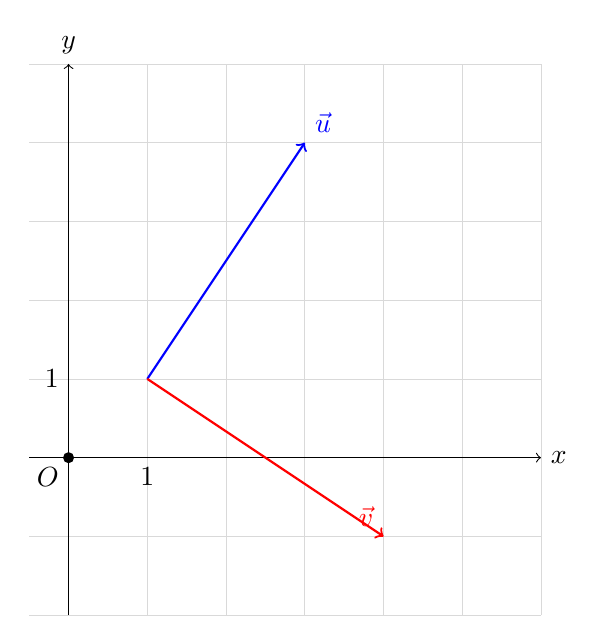
\begin{tikzpicture}[scale=1]

% Grille
\draw[step=1cm,gray!30,very thin] (-0.5,-2) grid (6,5);

% Axes
\draw[->] (-0.5,0) -- (6,0) node[right] {$x$};
\draw[->] (0,-2) -- (0,5) node[above] {$y$};

% Origine
\fill (0,0) circle (2pt) node[below left] {$O$};

% Graduation
\draw (1,0) node[below]{1};
\draw (0,1) node[left]{1};

% Vecteur u
\draw[->, thick, blue] (1,1) -- (3,4) node[above right] {$\vec{u}$};

% Vecteur v
\draw[->, thick, red] (1,1) -- (4,-1) node[above left] {$\vec{v}$};

\end{tikzpicture}
\end{center}
On constate que le vecteur $\vec{v}\pvec{3}{-2}$ convient. 
On fait donc l'hypothèse que, dans le cas général $\vec{v} \pvec{y}{-x}$ convient (à noter que $\vec{v} \pvec{-y}{x}$ convient aussi).
Cette hypothèse pourra être confirmée avec un outil permettant de mesurer les angles : le produit scalaire.
}

%%%%%%%%%%%%% SUJET B %%%%%%%%%%%%%%
\setcounter{Exercise}{0}
\newpage

\pagestyle{fancy}
\fancyhead[L]{Seconde}
\fancyhead[C]{\textbf{DS n°7b - Vecteurs}}
\fancyhead[R]{\today}

\null\vspace{-30pt}
Nom / Prénom : \\

Consignes particulières : 
\begin{itemize}[label=$\bullet$]
	\item 
	La calculatrice est \textbf{interdite}.
		\item 
	L'exercice \ref{exe:cours_b} peut être fait entièrement sur la feuille d'évaluation. 
	Écrire son nom avant de rendre le sujet pour qu'il soit corrigé.
	\item 
	Toute trace de recherche est prise en compte.
	%\item 
	%L'abbréviation $\tq$ signifie ``tel que''.
\end{itemize}

\hrule
\null\vspace{10pt}
Sauf mention contraire, on se place toujours dans un repère $(O, \vec{i}, \vec{j})$.

\exe{3}{
On donne $\vec{u}\pvec{3}{6}, \vec{v}\pvec{1}{-2}$ et $\vec{w}\pvec{2}{8}$. Compléter les phrases ci-dessous.
\begin{enumerate}[label=(\roman*),itemsep=5pt]
\item $\dfrac13 \vec{u} \pvec{\dots \dots}{\dots \dots}$ ;
\item $(\vec{u} - \vec{v}) \pvec{\dots \dots}{\dots \dots}$ ;
\item Les vecteurs $\vec{u}$ et $\vec{w}$ sont $\dots \dots$.
\end{enumerate}
}{exe:cours_b}{
\begin{enumerate}[label=(\roman*),itemsep=5pt]
\item $\dfrac13 \vec{u} \pvec{1}{2}$ ;
\item $(\vec{u} - \vec{v}) \pvec{2}{8}$ ;
\item Les vecteurs $\vec{u}$ et $\vec{w}$ sont non colinéaires (ou encore inégaux, de directions différentes, etc.).
\end{enumerate}
}

\exe{2}{
On considère les points $A(5;2), B(3;5), C(-1;4)$ et $D(-3;7)$.
Calculer les coordonnées des vecteurs $\vec{AB}$ et $\vec{CD}$. En déduire la nature du quadrilatère $ABCD$.
}{exe:pme1_b}{
On a $\vec{AB} \pvec{-2}{3}$ et $\vec{CD}\pvec{-2}{3}, \vec{AB} = \vec{CD}$ donc $ABCD$ est un parallélogramme.
}

\exe{2}{
Donner les coordonnées des vecteurs ci-dessous :

\begin{center}
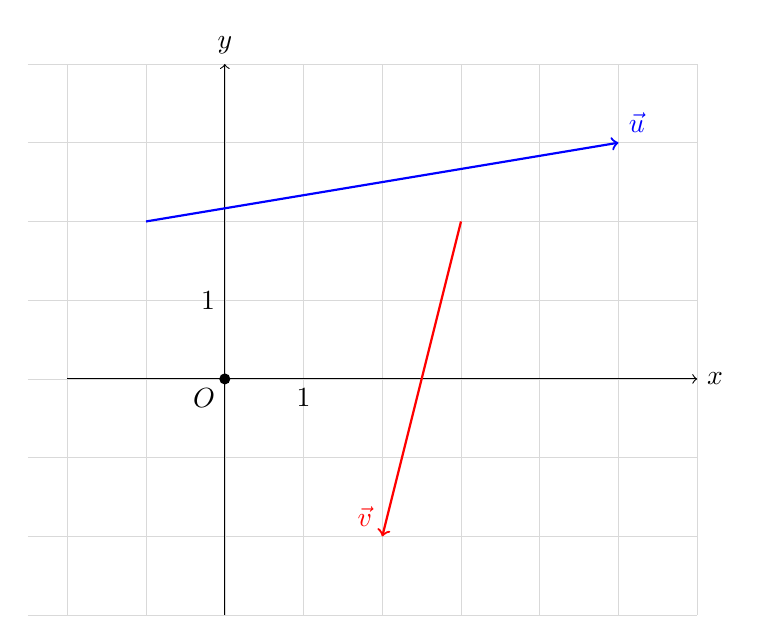
\begin{tikzpicture}[scale=1]

% Grille
\draw[step=1cm,gray!30,very thin] (-2.5,-3) grid (6,4);

% Axes
\draw[->] (-2,0) -- (6,0) node[right] {$x$};
\draw[->] (0,-3) -- (0,4) node[above] {$y$};

% Origine
\fill (0,0) circle (2pt) node[below left] {$O$};

% Graduation
\draw (1,0) node[below]{1};
\draw (0,1) node[left]{1};

% Vecteur u
\draw[->, thick, blue] (-1,2) -- (5,3) node[above right] {$\vec{u}$};

% Vecteur v
\draw[->, thick, red] (3,2) -- (2,-2) node[above left] {$\vec{v}$};

\end{tikzpicture}
\end{center}

}{exe:coord_b}{
$\vec{u}\pvec{6}{1}, \vec{v}\pvec{-1}{-4}$
}

% récup manuel Magnard 2019
\exe{4}{
Soient $A, B$ et $C$ trois points non alignés. On construit les points $M, N$ et $P$ tels que :
\[ \vec{AM} = \dfrac13 \vec{AB} \qquad \vec{CN} = \dfrac13 \vec{CA} \et \vec{CP} = \dfrac13 \vec{BC} \]
\begin{enumerate}
\item Réaliser une figure ;
\item Exprimer $\vec{MN}$ en fonction de $\vec{BA}$ et $\vec{AC}$.
\item Exprimer $\vec{MP}$ en fonction de $\vec{BA}$ et $\vec{AC}$.
\item En déduire que les points $M, N$ et $P$ sont alignés.
\end{enumerate}
}{exe:chasles_b}{
Voir correction sujet a.
}

\exe{2}{
Dans chaque cas ci-dessous, déterminer si les droites $(AB)$ et $(CD)$ sont parallèles :
\begin{enumerate}[label=(\roman*)]
\item $A(-4;5), B(1; 3), C(2 ; -7)$ et $D(-2 ; -5)$ ;
\item $A(1; -5), B(-3;9), C(2 ; 2)$ et $D(0 ; 9)$   
\end{enumerate}
}{exe:det1_b}{
\begin{enumerate}[label=(\roman*)]
\item $\vec{AB}\pvec{5}{-2}$ et $\vec{CD}\pvec{-4}{2}$ donc $\det{\vec{AB}, \vec{CD}}=2$, les droites $(AB)$ et $(CD)$ ne sont pas
parallèles.
\item $\vec{AB}\pvec{-4}{14}$ et $\vec{CD}\pvec{-2}{7}$ donc $\det{\vec{AB}, \vec{CD}}=0$, les droites $(AB)$ et $(CD)$ sont parallèles.
\end{enumerate}
}

\exe{2}{
Dans chaque cas ci-dessous, déterminer si les points $A, B$ et $C$ sont alignés.
\begin{enumerate}[label=(\roman*)]
\item $A(-1;-4), B(2; 2)$ et $C(4 ; 6)$ ;
\item $A(5;-2), B(-1 ; 1)$ et $C(-7, 2)$. 
\end{enumerate}
}{exe:det2_b}{
\begin{enumerate}[label=(\roman*)]
\item $\vec{AB}\pvec{3}{6}$ et $\vec{BC}\pvec{2}{4}$ donc $\det{\vec{AB}, \vec{BC}}=0$, les points $A, B$ et $C$ sont alignés.
\item $\vec{AB}\pvec{-6}{3}$ et $\vec{BC}\pvec{-6}{1}$ donc $\det{\vec{AB}, \vec{BC}}=12$, les points $A, B$ et $C$ ne sont pas alignés.
\end{enumerate}
}

\exe{3}{
On donne $\vec{u}\pvec{3}{4}$.
\begin{enumerate}
\item Calculer la norme du vecteur $\vec{u}$.
\item Calculer la norme du vecteur $\dfrac15 \vec{u}$.
\item Soit $\vec{v} \pvec{1}{1}$. 
En vous inspirant de la question précédente, proposer un nombre $k \in \R$ tel que $\norm{k \vec{v}} = 1$.
\end{enumerate}
\textit{Ce procédé est appelé \og normalisation d'un vecteur \fg}.
}{exe:norm1}{
\begin{enumerate}
\item On trouve $\norm{\vec{u}} = \sqrt{3^2+4^2} = \sqrt{25} = 5$.
\item Selon la propriété du cours $\dfrac15 \vec{u} = 1$.
\item Comme $\norm{\vec{v}} = \sqrt{2}$, on propose $k = \dfrac{1}{\sqrt{2}}$.
\end{enumerate}
}

\exe{2}{
On considère les points $P(7;-8), Q(-4;4)$ et $R(3;6)$.
Déterminer les coordonnées du point $S$ tel que $PQRS$ soit un parallélogramme.
}{exe:pme2_b}{
On pose $S(x;y)$. On a $\vec{PQ}\pvec{-11}{12}$. On veut que $\vec{SR} = \vec{PQ}$ avec $\vec{SR}\pvec{3-x}{6-y}$.
On résoud le système :
\[ \left \{ \begin{array}{c c}
3 - x & = -11 \\
6 - y & = 12
\end{array} \right. \]
et on trouve $S(14 ; -6)$.
}

\exe{}{
(Bonus) \\
Soit $\vec{u} \pvec{x}{y}$ un vecteur quelconque. Donner une expression générale (i.e. en fonction de $x$ et $y$) des coordonnées
du vecteur $\vec{v}$ afin que les vecteurs $\vec{u}$ et $\vec{v}$ soient orthogonaux (i.e. que leurs directions soient perpendiculaires). \\

\textit{Indication : on pourra essayer de procéder par tâtonnement en fixant des valeurs pour les variables $x$ et $y$ et en réalisant
des figures.}
}{exe:bonus_b}{
Voir correction sujet a.
}

%%%%%%%%%%%%

\newpage
\fancyhead[C]{\textbf{Solutions}}
Les solutions sont données dans l'ordre, sujet a puis sujet b.
\shipoutAnswer

\end{document}
